\documentclass[a4paper, twoside]{report}

\usepackage[english]{babel}
\usepackage[utf8]{inputenc}
\usepackage[T1]{fontenc}
\usepackage{listings}
\usepackage{hyperref}
\hypersetup{colorlinks=false}
\usepackage{lscape}
\usepackage{subfigure}
\usepackage{amsmath}
\usepackage{graphicx}
\usepackage[colorinlistoftodos]{todonotes}
\usepackage[backend=biber]{biblatex}

\DeclareMathOperator{\relu}{ReLU}
\DeclareMathOperator{\softmax}{softmax}

\addbibresource{bibs/references.bib}

%% Sets page size and margins
\usepackage[a4paper,top=3cm,bottom=2cm,left=3cm,right=3cm,marginparwidth=1.75cm]{geometry} 

\title{Semi-supervised graph node classification of CORA dataset using GCN}
\author{Junghyun Lee}
% Update supervisor and other title stuff in title/title.tex

\begin{document}
\begin{titlepage}

\newcommand{\HRule}{\rule{\linewidth}{0.5mm}} % Defines a new command for the horizontal lines, change thickness here

%----------------------------------------------------------------------------------------
%	LOGO SECTION
%----------------------------------------------------------------------------------------


\includegraphics[width=8cm]{title/logo.png}\\[1cm] % Include a department/university logo - this will require the graphicx package
 
%----------------------------------------------------------------------------------------

\center % Center everything on the page

%----------------------------------------------------------------------------------------
%	HEADING SECTIONS
%----------------------------------------------------------------------------------------
\quad\\[1.5cm]
%\textsc{\LARGE MSc Thesis}\\[1.5cm] % Name of your university/college
\textsc{\Large Korea Advanced Institute of Technology}\\[0.5cm] % Major heading such as course name
\textsc{\large Department of Mathematical Sciences}\\[0.5cm] % Minor heading such as course title

%----------------------------------------------------------------------------------------
%	TITLE SECTION
%----------------------------------------------------------------------------------------
\makeatletter
\HRule \\[0.4cm]
{ \huge \bfseries \@title}\\[0.4cm] % Title of your document
\HRule \\[1.5cm]
 
%----------------------------------------------------------------------------------------
%	AUTHOR SECTION
%----------------------------------------------------------------------------------------

\begin{minipage}{0.4\textwidth}
\begin{flushleft} \large
\emph{Author:}\\
\@author % Your name
\end{flushleft}
\end{minipage}
~
\begin{minipage}{0.4\textwidth}
\begin{flushright} \large
\emph{Instructor:} \\
Prof. Chang Dong Yoo 
% Uncomment the following lines if there's a co-supervisor
%\\[1.2em] % Supervisor's Name
%\emph{Co-Supervisor:} \\
%Dr. Adam Smith % second marker's name
\end{flushright}
\end{minipage}\\[3cm]
\makeatother


%----------------------------------------------------------------------------------------
%	DATE SECTION
%----------------------------------------------------------------------------------------

{\large Final Project - Graph}\\[0.5cm]
{\large \emph{EE531: Statistical Learning Theory, Fall 2019}}\\[0.5cm]
{\large \today}\\[2cm] % Date, change the \today to a set date if you want to be precise

\vfill % Fill the rest of the page with whitespace

\end{titlepage}

\begin{abstract}
In this homework, I have implemented a simple version of GCN(Graph Convolutional Network) to do a semi-supervised graph node classification of CORA dataset.
The algorithm is based upon the work by Kipf \& Welling, 2016.

(Coding done in Google Colaboratory.)
\end{abstract}
 
\tableofcontents

\chapter{Background}
The background section of the dissertation should set the project into context by relating it to existing published work which you read at the start of the project when your approach and methods were being considered. There are usually many ways of solving a given problem, and you shouldn't just pick one at random. Describe and evaluate as many alternative approaches as possible. The background section is often included as part of the introduction but can be a separate chapter if the project involved an extensive amount of research.

The published work may be in the form of research papers, articles, text books, technical manuals, or even existing software or hardware of which you have had hands-on experience. Don't be afraid to acknowledge the sources of your inspiration; you are expected to have seen and thought about other people's ideas; your contribution will be putting them into practice in some other context. However, you must avoid plagiarism: if you take another person's work as your own and do not cite your sources of information/inspiration you are being dishonest; in other words you are cheating.
\chapter{Results}
%For my evaluation, I've used {\bf Tensorboard} for plotting the learning(loss) curve and performance(accuracy) curve for both training and validating processes. Also, I've used external open source library({\bf pretty-print-confusion-matrix}\footnote{\url{https://github.com/wcipriano/pretty-print-confusion-matrix}}) for plotting the confusion matrix for the test set.
Here,
\begin{itemize}
\item Original model: One with uniform initialization with dropouts(rate=0.5).

\item Ver. 1: Original model with Xavier (Uniform) Initialization

\item Ver. 2: Original model without dropouts

\item Ver. 3: Original model with Xavier Initialization and without dropouts
\end{itemize}

In all the plots, x-axis corresponds to the epoch.
As for the graphs,

\begin{itemize}
\item Accuracy graph
	\begin{itemize}
	\item Dark red: train accuracy
	\item Bright red: validation accuracy
	\end{itemize}

\item Loss graph
	\begin{itemize}
	\item Dark blue: train loss
	\item Bright blue: validation loss
	\end{itemize}
\end{itemize}

\newpage
\section{Original model}

\begin{figure}[htbp]
\centering
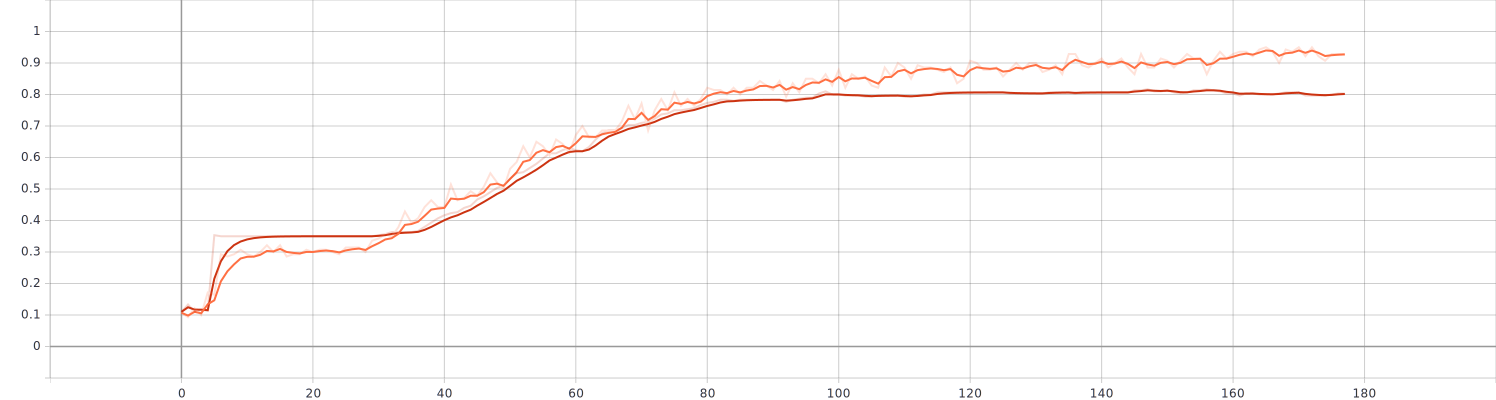
\includegraphics[width=0.7\linewidth]{results/fig/Accuracy0.png}
\caption{Accuracy graph}
\label{fig:accuracy0}
\end{figure}

\begin{figure}[htbp]
\centering
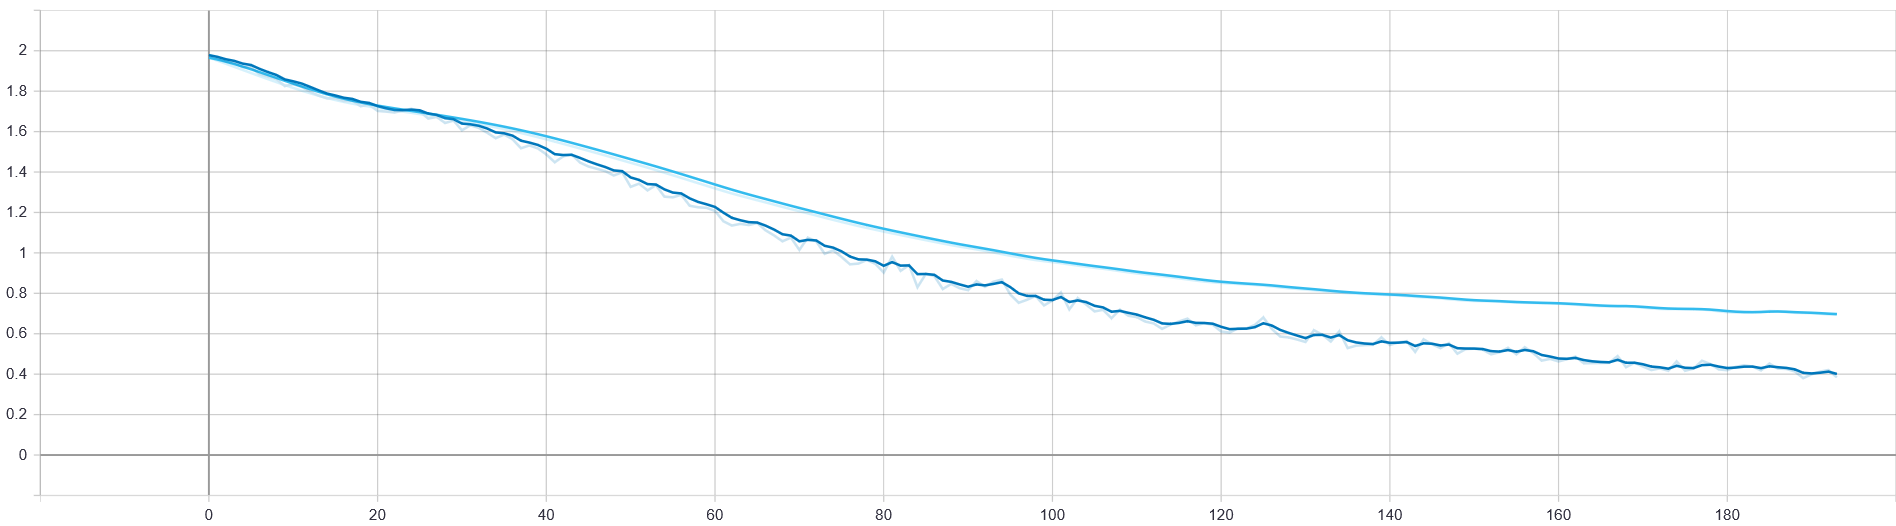
\includegraphics[width=0.7\linewidth]{results/fig/Loss0.png}
\caption{Loss graph}
\label{fig:evaluation0}
\end{figure}

\begin{figure}[htbp]
\centering
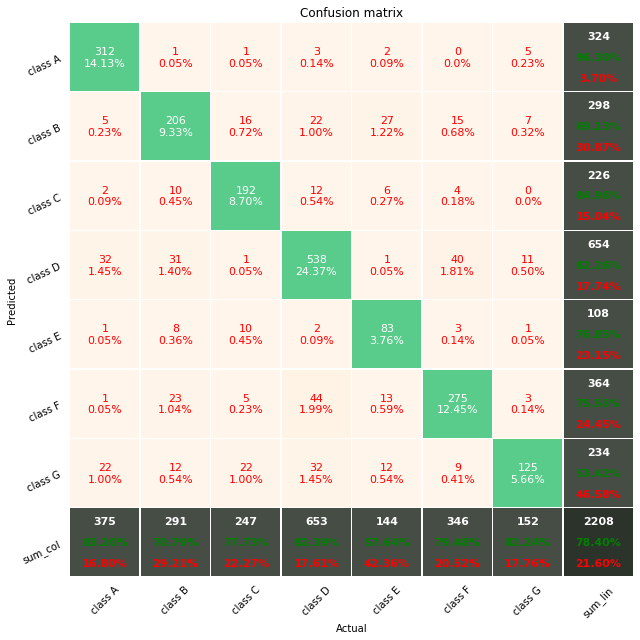
\includegraphics[width=0.6\linewidth]{results/fig/confusion0.png}
\caption{Confusion matrix}
\label{fig:confusion0}
\end{figure}

\newpage
\section{Modified Model (Ver. 1)}

\begin{figure}[htbp]
\centering
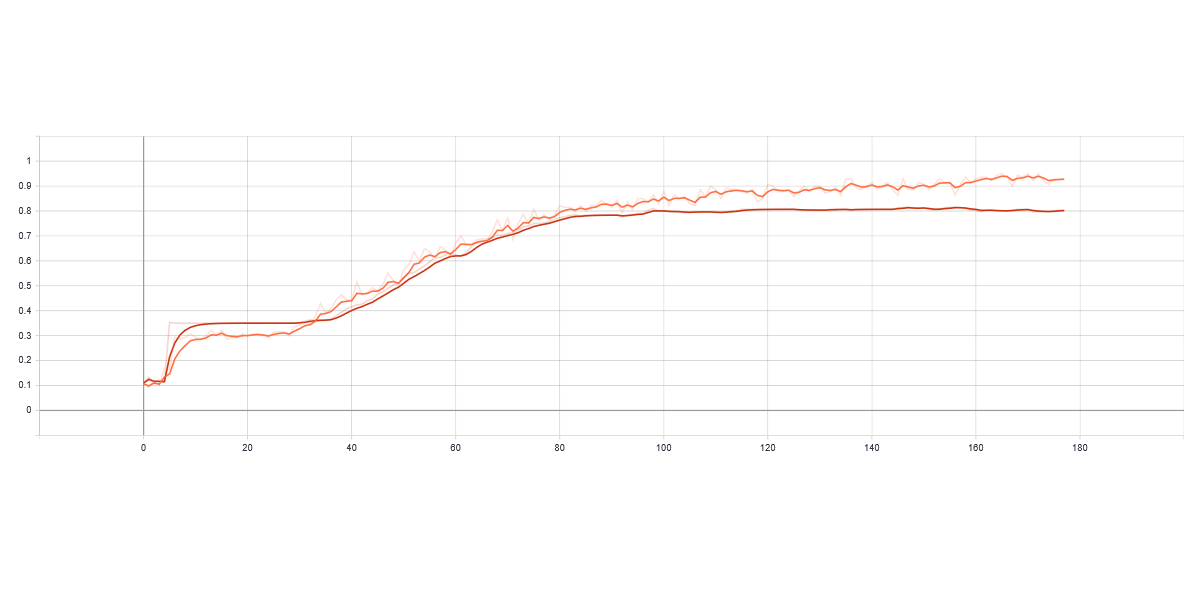
\includegraphics[width=0.7\linewidth]{results/fig/Accuracy1.png}
\caption{Accuracy graph}
\label{fig:accuracy1}
\end{figure}

\begin{figure}[htbp]
\centering
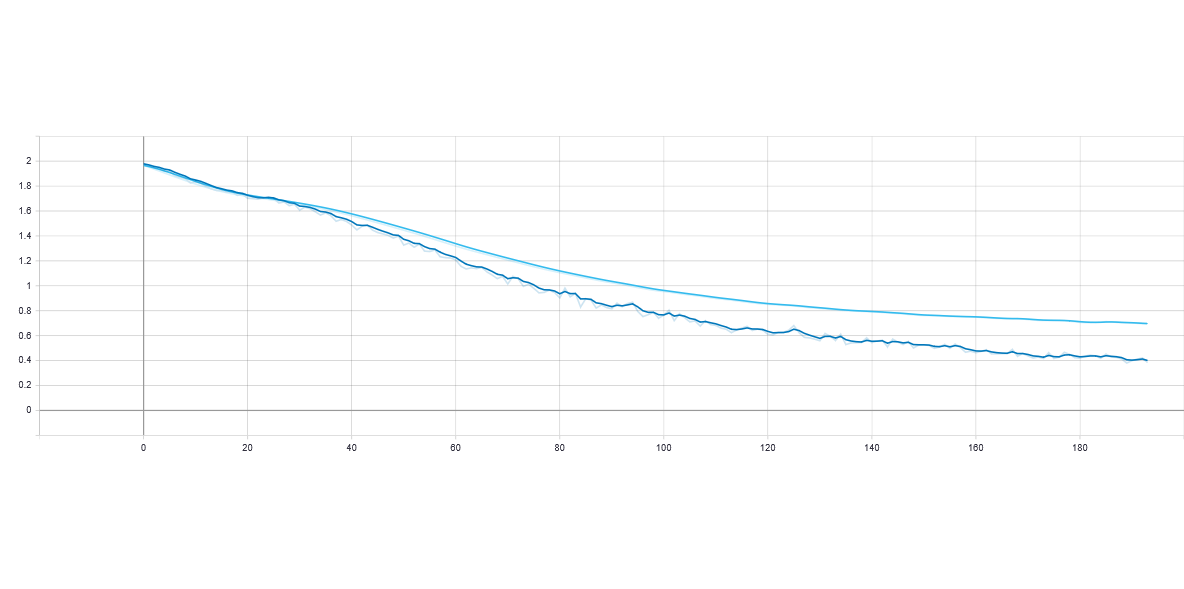
\includegraphics[width=0.7\linewidth]{results/fig/Loss1.png}
\caption{Loss graph}
\label{fig:evaluation1}
\end{figure}

\begin{figure}[htbp]
\centering
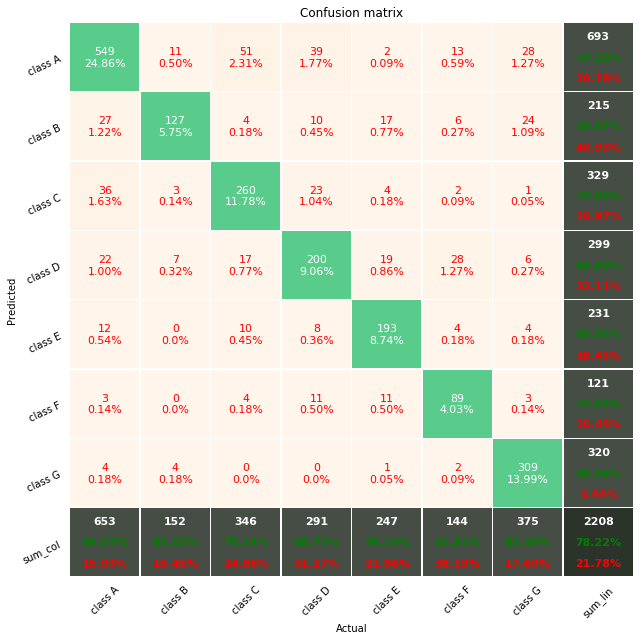
\includegraphics[width=0.6\linewidth]{results/fig/confusion1.png}
\caption{Confusion matrix}
\label{fig:confusion1}
\end{figure}

\newpage
\section{Modified Model (Ver. 2)}

\begin{figure}[htbp]
\centering
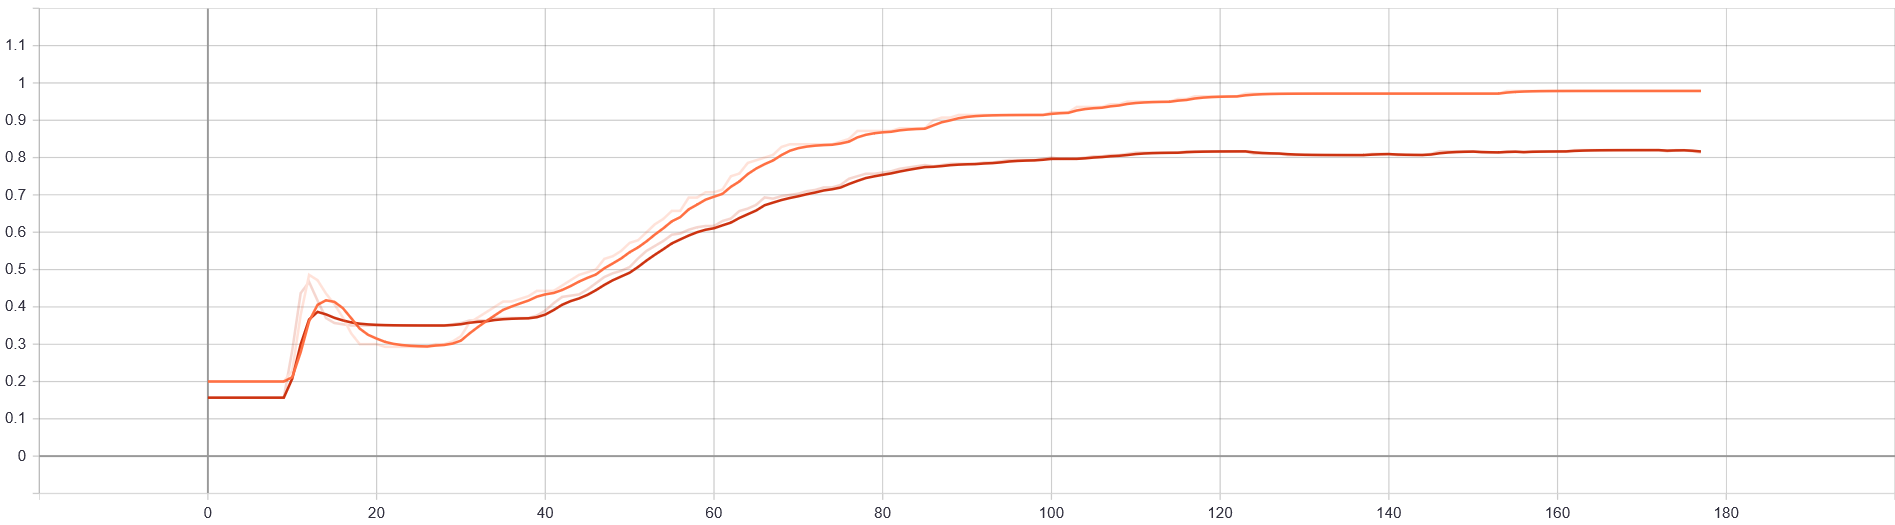
\includegraphics[width=0.7\linewidth]{results/fig/Accuracy2.png}
\caption{Accuracy graph}
\label{fig:accuracy2}
\end{figure}

\begin{figure}[htbp]
\centering
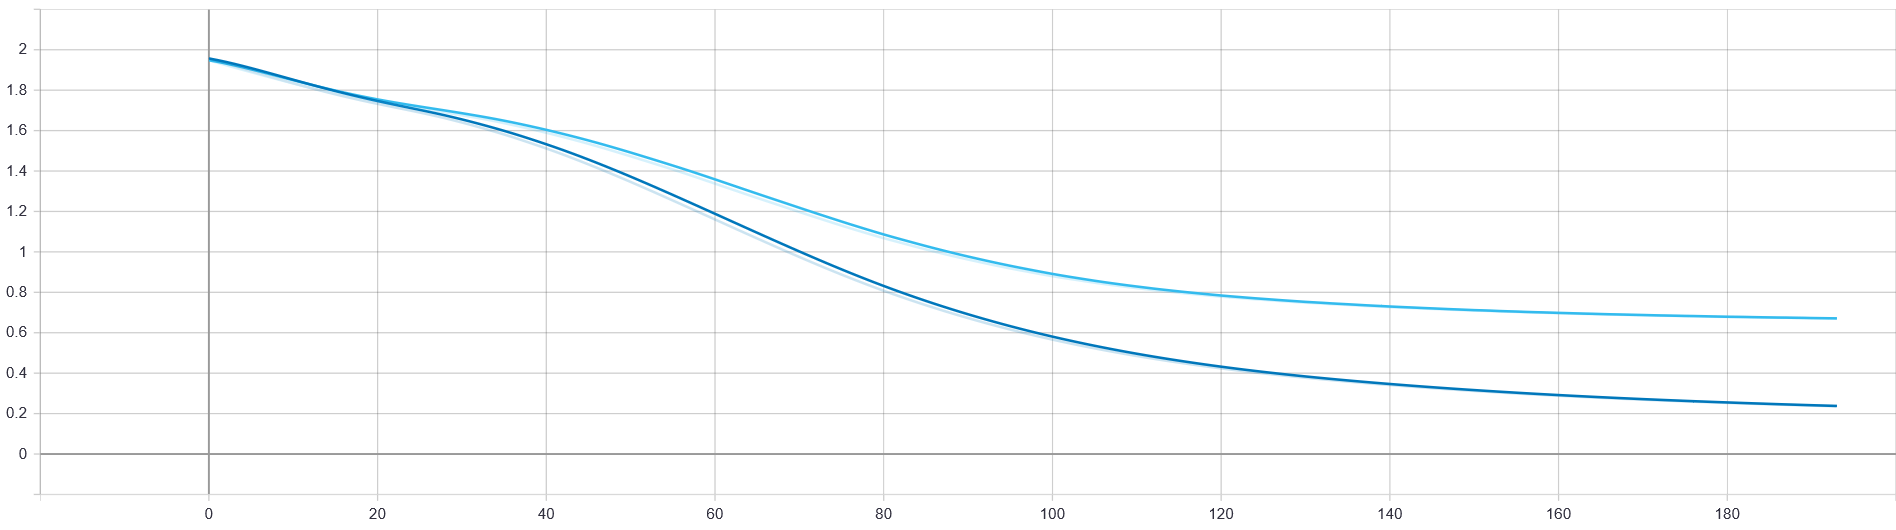
\includegraphics[width=0.7\linewidth]{results/fig/Loss2.png}
\caption{Loss graph}
\label{fig:evaluation2}
\end{figure}

\begin{figure}[htbp]
\centering
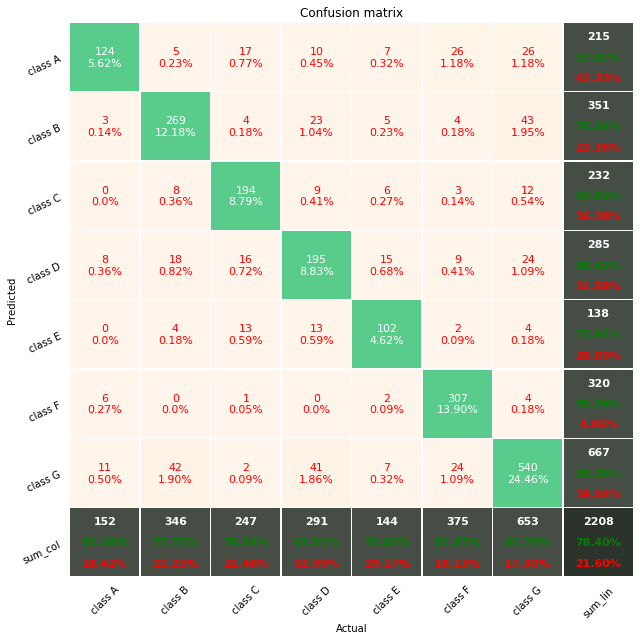
\includegraphics[width=0.6\linewidth]{results/fig/confusion2.png}
\caption{Confusion matrix}
\label{fig:confusion2}
\end{figure}

\newpage
\section{Modified Model (Ver. 3)}

\begin{figure}[htbp]
\centering
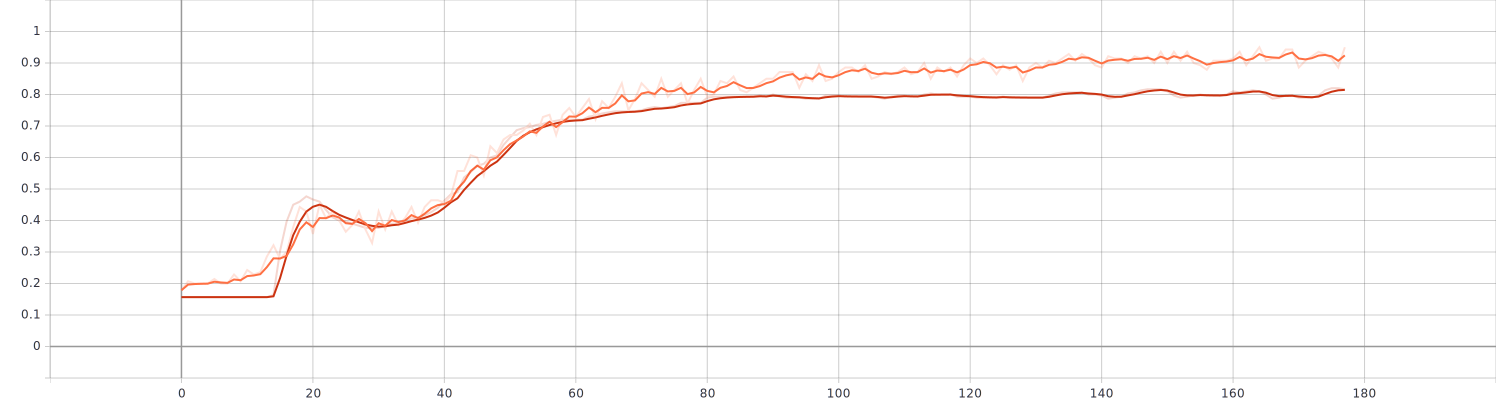
\includegraphics[width=0.7\linewidth]{results/fig/Accuracy3.png}
\caption{Accuracy graph}
\label{fig:accuracy3}
\end{figure}

\begin{figure}[htbp]
\centering
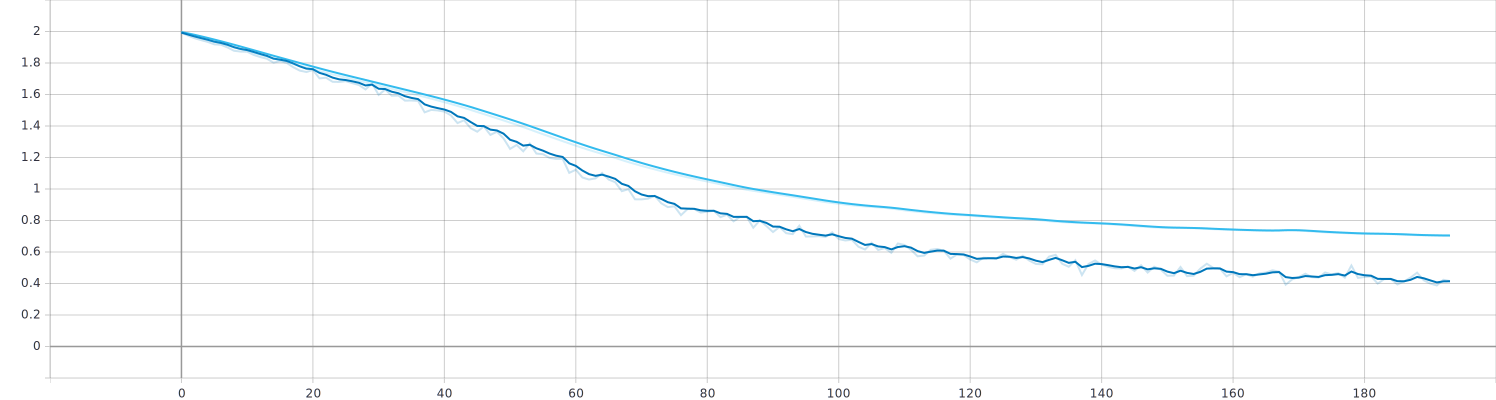
\includegraphics[width=0.7\linewidth]{results/fig/Loss3.png}
\caption{Loss graph}
\label{fig:evaluation3}
\end{figure}

\begin{figure}[htbp]
\centering
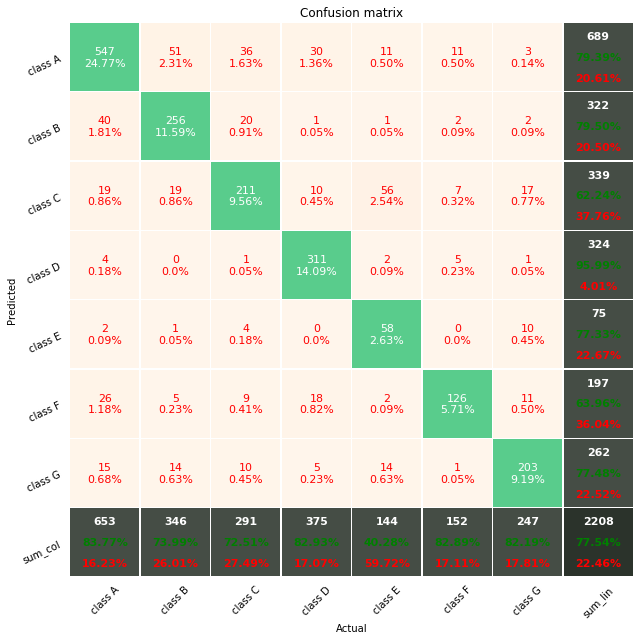
\includegraphics[width=0.6\linewidth]{results/fig/confusion3.png}
\caption{Confusion matrix}
\label{fig:confusion3}
\end{figure}

\chapter{Conclusion}

\notecite{}
\printbibliography 
%\bibliographystyle{unsrt}
%\bibliography{bibs/references}
\addcontentsline{toc}{chapter}{Bibliography}

\end{document}